%\documentclass[a4paper]{article}
\documentclass[12pt,letterpaper,final]{article}
\topmargin-2cm
\oddsidemargin0cm
\evensidemargin0cm
\textheight23cm
\textwidth16cm


\usepackage{textcomp}
\usepackage{listings}
\usepackage{amssymb}
\usepackage{amsmath}
\usepackage{url}
\usepackage{graphicx}
\usepackage[all]{xy}
\usepackage{pstricks}


\lstset{xleftmargin=1cm}

\newcommand{\x}{\boldsymbol{x}}
\newcommand{\xh}{\widehat{\boldsymbol{x}}}
\newcommand{\y}{\boldsymbol{y}}
\newcommand{\z}{\boldsymbol{z}}
\newcommand{\zero}{\boldsymbol{0}}
\newcommand{\dd}{\boldsymbol{d}}
\newcommand{\hdd}{\widehat{\dd}}

\newcommand{\bbR}{\mathbb{R}}
\newcommand{\bbC}{\mathbb{C}}
\newcommand{\bbN}{\mathbb{N}}

\newcommand{\et}{\widetilde{e}}

\newcommand{\surface}{\partial D}

\newcommand{\inc}{\mathrm{inc}}

\setlength{\parindent}{0cm}
\setlength{\parskip}{3ex}

\newtheorem{example}{Example}

\newcommand{\techheading}[1]{%
    \par\vspace{-0.3\parskip}\noindent\hspace{-1cm}\textbf{#1}%
    \par\vspace{-0.5\parskip}\noindent\nopagebreak\ignorespaces}

%\newenvironment{mylisting}{\begin{lstlisting}[language=matlab,basicstyle=\ttfamily,belowskip=-0.3 \baselineskip]}{\end{lstlisting}}

%\newenvironment{mylisting}{\begin{lstlisting}}{\end{lstlisting}}

\lstnewenvironment{matlab}{\lstset{language=matlab,basicstyle=\ttfamily,commentstyle=\ttfamily,belowskip=-0.3 \baselineskip,columns=fullflexible,upquote=true}}{}

\lstnewenvironment{unix}{\lstset{language=bash,basicstyle=\ttfamily,belowskip=-0.4 \baselineskip,columns=fullflexible}}{}

\lstnewenvironment{dos}{\lstset{language=dos,basicstyle=\ttfamily,belowskip=-0.3 \baselineskip,columns=fullflexible}}{}

\lstMakeShortInline[language=matlab,basicstyle=\ttfamily,belowskip=-0.3 \baselineskip]!

\bibliographystyle{plain}

\begin{document}
\title{{\bf TMATROM}:\\object-oriented  T-MATrix Reduced Order Model software
for efficient simulation of multi-parameter acoustic scattering}


\author{%
M. Ganesh,\\ Department of Applied Mathematics and Statistics,\\ Colorado School of Mines, Golden, CO 80401, USA \\
{\tt mganesh@mines.edu}
\and
Stuart C. Hawkins,\\ Department of Mathematics,\\Macquarie University, Sydney, NSW 2109, Australia \\
{\tt stuart.hawkins@mq.edu.au}}
\date{}

\maketitle

\vspace{-0.55in}
\begin{abstract}

\vspace{-0.2in}
Efficient simulation of scattering cross sections of wave scattering configurations
is an important tool for several applications. The transition matrix (T-matrix) based approach, that is 
independent of certain input parameters, provides an efficient framework for scattering simulations
with varying parameters in the configurations, including dynamic and uncertain configurations.  
In recent years, the authors developed and mathematically analyzed  a numerically stable T-matrix approach,
solving a several decade open problem of  developing {\em a priori} T-matrix truncation parameters that are 
independent of the shape of the particle. We develop and describe details of  an
associated computational counterpart that will provide an open-source software package for simulation of multi-parameter acoustic scattering models.


In this article, we describe an object oriented  software package TMATROM which provides a class of reduced order model (ROM) tools for efficient simulation of
multi-parameter acoustic scattering by obstacles in two dimensions.
Such multi-parameter problems occur, for example,  in monostatic cross section computations (involving
thousands of input incident directions),  in stochastic computations, and in multiple scattering simulations.
The TMATROM package provides offline tools for computing the T-matrix of
any two dimensional obstacle using {\em any} forward wave propagation solver.
Example solvers based on the Nystr\"om method are provided along with a framework to
add any other solver.  The TMATROM package provides efficient and easy to use online tools for 
quickly solving multi-parameter scattering problems.
Detailed examples are provided within the software package for monostatic cross section computations,
and multiple scattering simulations.
\end{abstract}

%\begin{figure}[ht!]
%\centering
%\vspace{-1cm}
%\begin{center}
%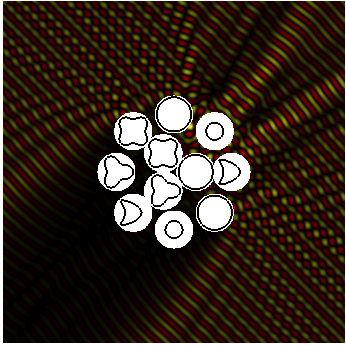
\includegraphics[width=12cm]{cover_multiple_total_field} 
%\end{center}
%\caption{\label{fig:multiple_cov_fig}}
%\end{figure}

\clearpage

\newpage
\section{Installation  and verification}
\vspace{-0.2in}

\techheading{Download }
Download the archive file !tmatrom.tar.gz! (Linux/Unix/OS X)
or !tmatrom.zip!. \\ (Contact the authors for  details of   downloading  the current version of the software.)
%from 
%\begin{displaymath}
%\mbox{\url{http://www.mines.edu/~mganesh/tmatrom}}
%\mbox{\url{http://www.romapp.org/}}
%\end{displaymath}
%using the  credentials,  {\bf {username: tmatrom\_reviewer,  password: for\_tmatrom\_reviewer}}

\techheading{Unpack}
Your system may automatically unpack the archive file for you.
If your system does not automatically unpack the archive you can unpack it
using (Linux/Unix/OS X)
\begin{unix}
tar -xvzf tmatrom.tar.gz
\end{unix}
or by opening it with Winzip (Windows).

\techheading{Save unpacked software in a (TMATROM) directory}
We recommend you save the files unpacked from the archive in a directory.
Below we refer to this directory as the TMATROM root directory.
%For example (Linux/Unix/OS X) use
%\begin{unix}
%~/tmatrom
%\end{unix}
%or (Windows)
%\begin{unix}
%C:\tmatrom
%\end{unix}


\techheading{Add TMATROM subdirectories to Matlab path}
After starting Matlab from the TMATROM root directory, type the command 
\begin{matlab}
setpath_tmatrom
\end{matlab}

\techheading{Run example codes}
Several examples are included in the TMATROM software package. Example codes 
(in directories prefixed EXAMPLE and with file names starting with the string !example_!)  
provide a quick way to test and use 
the package before looking into details of the  objected-oriented ROM  in this article.

After installation, 
we recommend that users type the following two
commands in  Matlab
to test the installation of the TMATROM package. 
The  first command solves and visualizes a bistatic (single parameter) 
sound-soft scattering simulation.
The second command solves and visualizes the corresponding 
monostatic (multi-parameter)
simulation with
with $1000$ input incident waves.
\begin{matlab}
example_rom_nystrom_soundsoft_bistatic
example_rom_nystrom_soundsoft_monostatic
\end{matlab}
Before proceeding further, users may also like to try  
examples for scatterers with other material properties
by  replacing
!soundsoft! in the above commands with !soundhard! or !absorbing!. Source codes for these 
and additional examples, including multiple particle configurations,  are in the 
TMATROM subdirectory !EXAMPLE_ROM_NYSTROM_SOLVER!.

We recommend users follow
the quick start guide in Section~\ref{sec:start}
to learn more about how to use the package.



\tableofcontents




\section{Introduction}

We describe the use of our object-oriented Matlab 
software package TMATROM. 
This package provides a class of reduced order model (ROM) software tools for  simulation of
multi-parameter
acoustic scattering by obstacles in two dimensions. For details of various forward and inverse 
scattering models and associated applications, we refer to~\cite{colton:inverse} and extensive list of references therein. The forward scattering model is governed by the 
Helmholtz equation and a  set of parameters  that provides information of the full model,
such as the input incident wave that induces 
the scattered field, and how the output
quantities of interest (QoIs) are measured (with a receiver direction parameter). Typical QoIs 
from the model are the scattered and far fields, and the associated acoustic cross section (ACS) of
the scattering configuration~\cite{colton:inverse}. 

Our ROM~\cite{gh:tmat2d, ghh:tmatrix} provides  a
very efficient framework when the scattering model needs to be simulated for 
multiple sets of  parameters.   
Such multiple parameter sets  occur, for example,
when the QoI is the {\em monostatic}  ACS,  corresponding to the situation where the receiver direction
is opposite to the incident direction (backscattering) and the receiver direction parameter varies from
zero to 360 degrees. 




Our computationally stable T-matrix approach~\cite{gh:tmat2d, ghh:tmatrix}   is an optimization-free reduced basis framework to setup up a matrix that  characterizes the scattering properties of an obstacle.
The matrix is independent of the incident and receiver directions. If the location and orientation of
the obstacle are changed, the associated new T-matrix can be quickly computed using techniques based on the translation-addition
theorem and the old 
T-matrix of the obstacle for the original location and orientation.
The T-matrix  can  be used  any number of times to
simulate scattered and far-fields after  setting up  appropriate vector  representations of several input incident
fields. 

%Essentially, the QoIs in the model problem are obtained using the simple T-matrix and vector multiplication. 
%Setting up of each column of a T-matrix is independent of the other columns. We exploit this naturally
%parallel property (and other appropriate parallel tasks)   in the TMATROM package and provide the user with an option of faster  simulation of the model using multiple cores in a single compute node. The parallel 
%option in the TMATROM requires the Matlab Parallel Computing Toolbox on the compute node. 
 

Multiple sets of parameters also arise in multiple particle scattering configurations, 
where the location and orientation of each particle in the configuration should be treated as parameters. 
The TMATROM framework is efficient
for the multiple particle configuration based scattering model, even
without prior knowledge of the location and orientation of each particle in the configuration, and
hence it is also appropriate for moving particle configurations. 

The TMATROM package provides an {\em offline} software framework to
build  a  T-matrix for any two dimensional obstacle with a user's choice of obstacle geometry and
appropriate material property (such as sound-soft, sound-hard, absorbing, penetrable).
Subsequently  the user  can efficiently develop an {\em online} approach 
by assembling various types of multiple particle deterministic or stochastic configurations~\cite{gh:stoc_mult}
comprising the obstacles. 



A major advantage of  our TMATROM framework is that it 
utilizes standard numerical methods for solving the scattering problem
(for a fixed parameter set)
{\em but}\,~it is
independent of  any 
specific numerical method.
Consequently, the TMATROM package  can be used in conjunction  with any existing 
forward wave propagation solver   that a user is already familiar with. 
Easy incorporation of  a solver into our object-oriented TMATROM core framework
requires only
that the solver can compute the far-fields associated with
incident  circular waves~\cite[Equation (2.15)]{ghh:tmatrix}.

To illustrate the easy customization of  our object-oriented framework,  
we
provide examples with 
two  distinct families of forward solvers with the TMATROM package.
The first is developed by 
the authors and uses the Nystr\"om method~\cite{colton:inverse}.
The second is based on an open-source forward solver using
non-polynomial finite elements and the method of fundamental 
solutions~\cite{mpspack:manual}. 
The forward solver
does not need to use Matlab's object-oriented framework, but 
it does need to use
the Matlab environment (and may use Mex files to incorporate procedures written using other
computer languages). 

% Later in this manual we describe a general approach   to incorporate any 
% user provided  Matlab based forward solver 
% %for a fixed set of the acoustic  
% %scattering model parameters 
% into our object-oriented framework. The authors will be happy to collaborate with any user or group to customize 
% their forward solver within our TMATROM framework. 

The package has two components.
The first component is the TMATROM kernel which contains object-oriented classes and functions
associated with the ROM. 
The kernel component is described in Part~\ref{part:core} of this manual.
The second component includes several example 
solvers for the scattering problem that will be
sufficient for most users. The example solvers are described in Part~\ref{part:provided-solvers}.
We will assume that the user is familiar with 
the basic features of Matlab.
The class structure of TMATROM is visualized in Figures~\ref{fig:wavefunctions}--\ref{fig:solvers}.

As described above, the TMATROM model is independent of the solver used and users
can provide their own solvers by extending templates provided.
Details required for coding user defined solvers
are described in Part~\ref{part:solvers-user}. 
In Part~\ref{part:solvers-user} we assume that the user is familiar with
object-oriented programming in Matlab.
The authors will be happy to collaborate with any user or group to customize 
their forward solver within our TMATROM framework. 

While we restrict the TMATROM package to the 2D models, our reduced basis T-matrix framework with {\em a priori} 
analytical truncation parameter estimates (without the expensive optimization techniques, such 
as the greedy approach, that are required in most reduced basis methods, see~\cite{ghs:12} and references therein) 
and exponential convergence analysis are applicable for both two and three dimensional 
scattering models~\cite{ghh:tmatrix}. In future we plan to develop a 3D version of the TMATROM package. 


{\em We request that any publications that make use of our TMATROM package cite 
our key papers on the ROM~\cite{gh:tmat2d, gh:stoc_mult, ghh:tmatrix} and this article}.
This article includes the minimal mathematical details required to understand
the underlying algorithm and the package can be used as a {\em black-box}
without knowledge of these details. For complete mathematical details of our stable ROM algorithm
and convergence analysis with application to stochastic multiple particle configurations,
we ask the user of this manual and TMATROM package to refer to~\cite{ghh:tmatrix}.


\begin{figure}[!ht]
\centering
\begin{displaymath}
\xymatrix{ \fbox{\texttt{wavefunctionexpansion}} & \\
\fbox{\texttt{radiatingwavefunctionexpansion}}\ar@/0ex/[u] &  \fbox{\texttt{radiatingwavefunctionexpansion}}\ar@/0ex/[ul]
}
\end{displaymath}
\caption{\label{fig:wavefunctions}
Figure showing the class dependencies for the wavefunction expansion classes.}
\end{figure}

\begin{figure}[!ht]
\centering
\begin{displaymath}
\xymatrix{ \fbox{\texttt{incident}} & & \\
\fbox{\texttt{wavefunction2d}}\ar@/0ex/[u] & \fbox{\texttt{plane\_wave}}\ar@/0ex/[ul] & \fbox{\texttt{point\_source}}\ar@/0ex/[ull] \\
\fbox{\texttt{regularwavefunction2d}}\ar@/0ex/[u] & \fbox{\texttt{radiatingwavefunction2d}}\ar@/0ex/[ul]
}
\end{displaymath}
\caption{\label{fig:incidents}
Figure showing the class dependencies for the incident wave classes.}
\end{figure}

\begin{figure}[!ht]
\centering
\begin{displaymath}
\xymatrix{ 
\fbox{\texttt{solver}} & & \fbox{\texttt{tmatrix}}\ar@{-->}[ll]_<<<1_>>>1 \\
\fbox{\texttt{solverNystrom}}\ar@/0ex/[u] & \fbox{\texttt{solverNystromRobin}}\ar@/0ex/[ul] & \fbox{\texttt{mfsExampleSolver}}\ar@/0ex/[ull] 
}
\end{displaymath}
\caption{\label{fig:solvers}
Figure showing the class dependencies for the solver and T-matrix classes.}
\end{figure}

\paragraph{A note on position vectors in TMATROM}

In our TMATROM code, and correspondingly in this manual,
we represent real valued vectors in $\bbR^2$ (such as position vectors) by 
complex numbers with the real part and imaginary parts of the complex number
corresponding
to the $x$- and $y$-coordinates of the vector respectively.

\section{Quick start guide}\label{sec:start}

In this section we first describe how to setup, simulate and visualize the scattered and far-field induced by  a plane wave impinging on a sound-soft kite shaped scatterer using the TMATROM package. 
Then, using the T-matrix of the kite scatterer, 
we demonstrate how to efficiently efficiently simulate  the monostatic ACS of the scatterer 
using hundreds of incident plane wave directions. 

First we setup the scatterer illustrated in Figure~\ref{fig:kite}:
\begin{matlab}
g = obstacleKite();
\end{matlab}

For a fixed wavenumber, say {\tt kwave = 1}, it requires only a few lines
(which are explained in detail later) to 
setup the incident wave direction independent T-matrix,
which exponentially accurately characterizes
the scattering properties of the scatterer:
\begin{matlab}
kwave = 1;
solver = solverNystrom(kwave,[],g);
solver.setup(15);
nmax = suggestedorder(kwave,solver.getRadius());
tmat = tmatrix(nmax,kwave,solver,0);
\end{matlab}
The dimension of the T-matrix is suggested by the wavelength 
of the problem and associated 
convergence analysis~\cite{ghh:tmatrix}.

A few more lines are required to simulate and visualize (see Figure~\ref{fig:kite_far_field}) the intensity of the far field 
induced by an incident plane wave with
direction $\hdd = (\cos \theta, \sin \theta)^T$ with, say,  $\theta = \pi/4$
impinging on the scatterer.
\begin{matlab}
p = plane_wave(pi/4,kwave);
b = tmat * regularwavefunctionexpansion(nmax,0,p);
b.visualizeFarField()
\end{matlab}

The monostatic ACS of the scatterer obtained at  $m = 1000$ (co-located transmitter and receiver)  angles in $[0, 2\pi]$
is easily and quickly simulated and visualized. 
\begin{matlab}
m = 1000;
farfield = zeros(m,1);
parfor j = 1:m
    p = plane_wave(pi+2*pi*j/m,kwave);
    c = tmat * regularwavefunctionexpansion(nmax,0,p);
    farfield(j) = c.evaluateFarField(exp(1i*2*pi*j/m));
end
plot(2*pi*(1:m)/m,10*log10(2*pi*abs(farfield).^2),'r')
\end{matlab}
The above commands will produce the plot in Figure~\ref{fig:kite_monostatic}.

\begin{figure}[!ht]
\centering
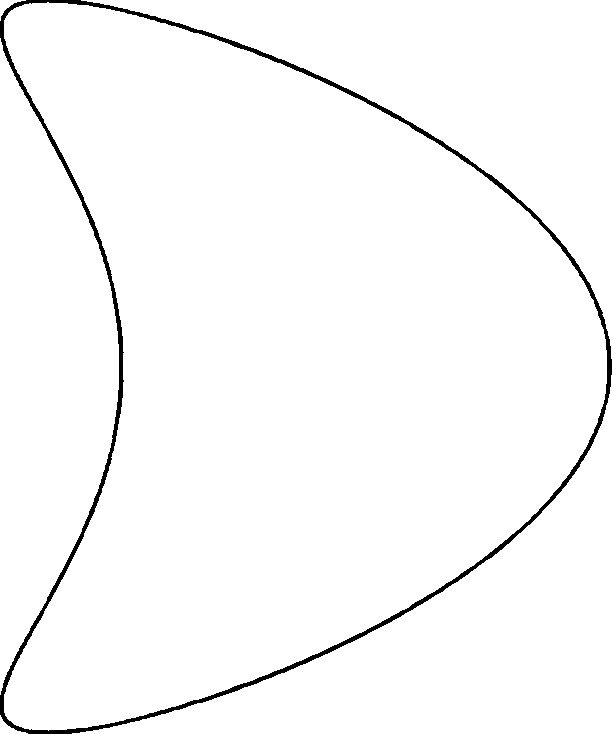
\includegraphics[width=5cm]{kite}
\caption{\label{fig:kite}
One of the TMATROM  built-in example scatterers: a kite shape.}
\end{figure}

\begin{figure}
\centering
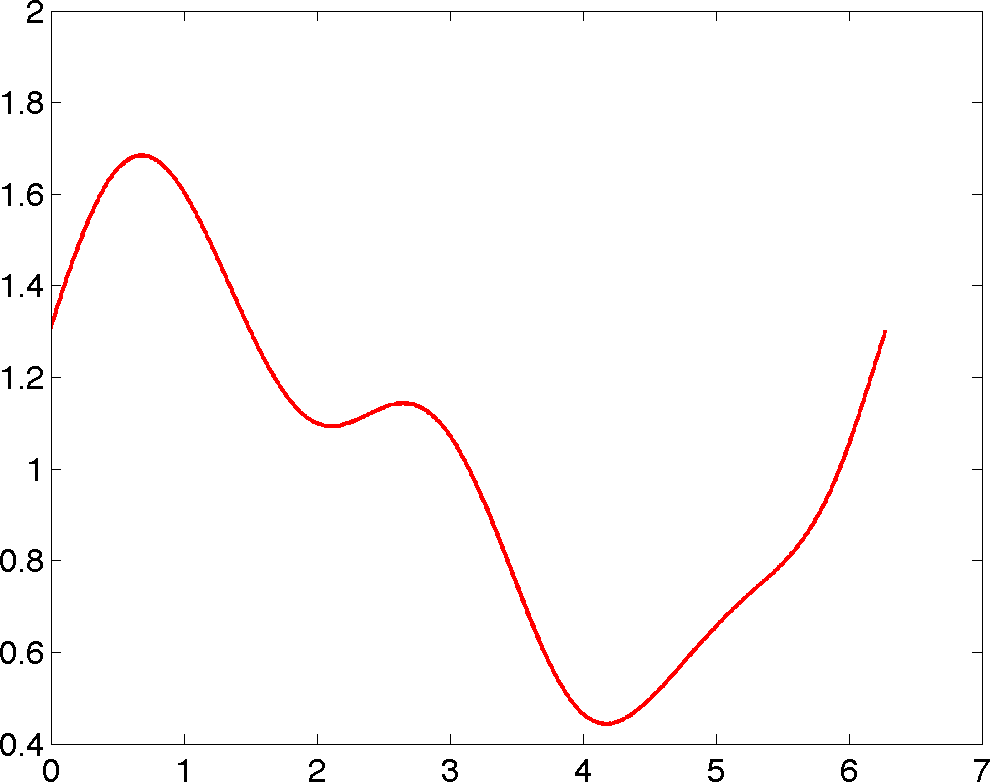
\includegraphics[width=10cm]{kite_far_field}
\caption{\label{fig:kite_far_field}
Absolute value of the far field induced by a plane wave   impinging  on the kite.}

\vspace{0.3in}
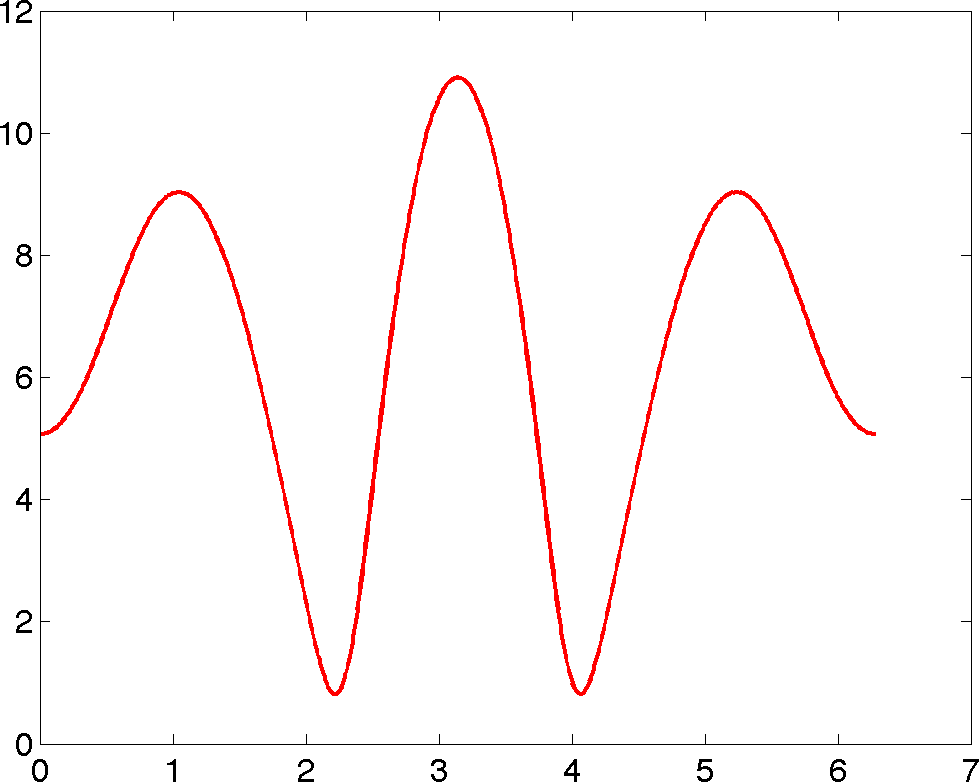
\includegraphics[width=10cm]{kite_monostatic_lowfreq_new_cartesian}
\caption{\label{fig:kite_monostatic}
Monostatic ACS  (dB) of the  kite shaped sound-soft scatterer 
simulated using $1000$ plane waves
with $1000$ incident direction angles in $[0, 2  \pi]$. }
\end{figure}

\newpage
\section{Mathematical Model}\label{sec:model}

In this section we briefly describe the exterior scattering problem,
in which an incident field interacts with a configuration to produce a scattered field.
The scattering configuration may comprise one or more obstacles 
with various material properties (for example sound hard, sound soft,
penetrable). In all cases, we denote the configuration by $D$. 

The incident wave may or not penetrate inside the obstacles in $D$.
In the case of a dielectric penetrable obstacle, the interior wavenumber
is different from the exterior wavenumber $k$; the 
medium inside the obstacle
may also be heterogeneous. 

The scattered field exterior to $D$  satisfies the constant coefficient 
Helmholtz equation~\cite{colton:inverse}
\begin{equation}
\label{eq:helmholtz}
\triangle u(\x) + k^2 u(\x) = 0, \qquad \x \in \bbR^2 \setminus \overline{D},
\end{equation}
and  the
Sommerfeld radiation condition~\cite[Equation~(3.85)]{colton:inverse}
\begin{equation}
\label{eq:radiation-condition}
\lim_{|\x| \to \infty} \sqrt{|\x|} \left(\frac{\partial u}{\partial \x}(\x) - ik u(\x) \right) = 0,
\end{equation}
uniformly as $|\x| \to \infty$. 
Here $k$ is the wavenumber of the incident field, which satisfies
%\begin{displaymath}
%$k = \frac{2 \pi}{\lambda}$, 
$k = 2 \pi / \lambda$, 
%\end{displaymath}
where $\lambda$ is the wavelength. 

For each impenetrable scatterer in $D$ the above system
needs to be augmented with a Dirichlet, Neumann, or Robin boundary condition, depending 
respectively on whether the obstacle is sound-soft or sound-hard or absorbing~\cite{colton:inverse, ghh:tmatrix}. 
For each penetrable scatterer in $D$ the above system 
needs to augmented with the interior 
(variable or constant coefficient) Helmholtz equation in the interior of the
obstacle
and an associated interface boundary condition on the obstacle surface.


The incident wave may be a plane wave
\begin{equation}
\label{eq:plane-wave}
u^\inc(\x) = e^{i k \x \cdot \hdd},
\end{equation}
with direction specified by the unit vector $\hdd$, or
a point source field
\begin{equation}
\label{eq:point-source}
u^\inc(\x) = H_0^{(1)} (k |\x - \y_0|),
\end{equation}
where $\y_0$ is the point source location.

In many problems
the quantities of interest (QoI) are  the  far field and associated
acoustic
cross section (ACS), in decibels (dB), 
as functions of the unit vectors $\xh = \x / |\x|$ 
(representing the observation or receiver directions), 
defined respectively as~\cite{colton:inverse, ghh:tmatrix}:
\begin{equation}
\label{eq:far-field}
u^\infty(\xh) = \lim_{|\x| \to \infty} \sqrt{|\x|} e^{-i k |\x|} u(\x), \qquad \qquad  
\sigma^{\mathrm{ACS}} (\xh) = 10\log_{10} (2\pi\left|u^\infty(\xh)\right|^2).
\end{equation}



\part{The core TMATROM classes}
\label{part:core}

Our T-matrix ROM~\cite{ghh:tmatrix} is based on expanding the regular incident 
field and the radiating scattered field using two distinct classes of basis functions. The
TMATROM package kernel 
provides associated object-oriented classes. The kernel is independent of
the solver used to simulate the mathematical model described in the previous section. 
\section{The \texttt{regularwavefunctionexpansion} class}

The regular circular  wavefunction with wavenumber $k$
\begin{equation}
\label{eq:regular-wavefunction}
\et_{\ell}(\z) = J_{|\ell|}(k |\z|) e^{i \ell \theta(\z)},
\end{equation}
satisfies the Helmholtz equation~(\ref{eq:helmholtz}) for all
$\z \in \bbR^2$.
Here $J_l$ denotes the Bessel function of order $l$ and
$(r,\theta) = (|\z|,\theta(\z))$ are polar coordinates for the point $\z$.
For fixed $n \in \bbN$ and coefficients $a_{-n},\dots,a_n$, the 
regular wavefunction series expansion
with origin $\x_0$,
\begin{equation}
\label{eq:regular-expansion}
u(\x) = \sum_{j=-n}^n a_j \et_j(\x - \x_0)
\end{equation}
is a regular solution of the Helmholtz equation~(\ref{eq:helmholtz}).

\techheading{Instantiation using coefficients}
The !regularwavefunctionexpansion! class represents regular
wavefunction expansions of the form~(\ref{eq:regular-expansion}).
Given a vector of coefficients !cof! of length $2 \texttt{n}+1$, 
an instance of the
!regularwavefunctionexpansion! class is created using
\begin{matlab}
u = regularwavefunctionexpansion(n,x0,k,cof);
\end{matlab}
where !k! is the wavenumber and !x0! is the expansion origin.
Here !cof(j)! contains the coefficient $a_{\texttt{j} - \texttt{n} -1}$
for $\texttt{j} = 1,\dots,2\texttt{n} + 1$.


\techheading{Instantiation from a plane wave}
If a function $u$ is regular in a neighbourhood of  $\x_0 \in \bbR^2$
then $u$ can be approximated by a regular wavefunction expansion of
the form~(\ref{eq:regular-expansion}).
If $u$ is a plane wave~(\ref{eq:plane-wave}) 
then there is an analytical expression for the coefficients~\cite{ghh:tmatrix}.
An instance of the !regularwavefunctionexpansion! class approximating
a !plane_wave! object !p! is created using
\begin{matlab}
u = regularwavefunctionexpansion(n,x0,p);
\end{matlab}
where !n! is the order of the expansion and !x0! is the expansion origin.

\techheading{Instantiation from a point source}
Similarly, if $u$ is the field induced by a point source~(\ref{eq:point-source})
there is an analytical expression for the coefficients~\cite{ghh:tmatrix}.
An instance of the !regularwavefunctionexpansion! class approximating
a !point_source! object !q! is created using
\begin{matlab}
u = regularwavefunctionexpansion(n,x0,q);
\end{matlab}
where !n! is the order of the expansion and !x0! is the expansion origin.
This expansion is valid only in neighbourhoods about !x0! 
that do not contain the point
source origin $\y_0$.

\techheading{Evaluation}
A !regularwavefunctionexpansion! object !u! is evaluated at points !z! using
\begin{matlab}
val = u.evaluate(z);
\end{matlab}
Here !z! may be a scalar, vector or matrix.
The !evaluate! method may be used to visualize the wavefunction expansion.
For example, to visualize !u! in 
$[-10, 10] \times [-10, 10]$ with $500 \times 500$ mesh points 
\begin{matlab}
t = linspace(-10,10,500);
[x,y] = meshgrid(t);
z = x + 1i*y;
surf(x,y,real(u.evaluate(z)))
\end{matlab}

\techheading{Visualization}
The !regularwavefunctionexpansion! class also provides a
convenient method for quickly visualizing the field. 
For example
\begin{matlab}
u.visualize([-10 10 -10 10])
\end{matlab}
produces a similar figure to the example above.

\techheading{Addition and subtraction}
Two !regularwavefunctionexpansion!s !u! and !v! 
that are compatible
are added using
\begin{matlab}
w = u + v;
\end{matlab}
and subtracted using
\begin{matlab}
w = u - v;
\end{matlab}
The !regularwavefunctionexpansion!s are compatible if they have the same
origins, wavenumbers and orders.

\section{The \texttt{radiatingwavefunctionexpansion} class}

The radiating wavefunction
\begin{equation}
\label{eq:radiating-wavefunction}
e_{l}(\z) = H^{(1)}_{|l|}(k |\z|) e^{i l \theta(\z)},
\end{equation}
satisfies the Helmholtz equation~(\ref{eq:helmholtz}) for all
$\z \in \bbR^2 \setminus \{ \zero \}$ and the radiation condition~(\ref{eq:radiation-condition}).
Here $H^{(1)}_l$ denotes the Hankel function of order $l$ and
$(r,\theta) = (|\z|,\theta(\z))$ are polar coordinates for the point $\z$.

For fixed $n \in \bbN$ and coefficients $b_{-n},\dots,b_n$, the 
radiating wavefunction series expansion
with origin $\x_0$,
\begin{equation}
\label{eq:radiating-expansion}
u(\x) = \sum_{m=-n}^n b_m e_m(\x - \x_0)
\end{equation}
is a radiating solution of the scattering problem~(\ref{eq:helmholtz})--(\ref{eq:radiation-condition}).

\techheading{Instantiation using coefficients}
The !radiatingwavefunctionexpansion! class represents radiating
wavefunction expansions of the form~(\ref{eq:radiating-expansion}).
Given a vector of coefficients !cof! of length $2 \texttt{n}+1$, an instance of the
!radiatingwavefunctionexpansion! class is created using
\begin{matlab}
u = radiatingwavefunctionexpansion(n,x0,k,cof);
\end{matlab}
where !k! is the wavenumber and !x0! is the expansion origin.
Here !cof(j)! contains the coefficient $b_{\texttt{j} - \texttt{n} -1}$
for $\texttt{j} = 1,\dots,2\texttt{n} + 1$.

Typically !radiatingwavefunctionexpansion! objects are created by
applying a transformation to a !regularwavefunctionexpansion! object.
This is described in detail in the next section.

\techheading{Evaluation}
A !radiatingwavefunctionexpansion! object !u! is evaluated at points !z! using
\begin{matlab}
val = u.evaluate(z);
\end{matlab}
Here !z! may be a scalar, vector or matrix.
The !evaluate! method may be used to visualize the wavefunction expansion.
For example to visualize !u! 
in $[-10, 10] \times [-10, 10]$ with $500 \times 500$ mesh points, 
\begin{matlab}
t = linspace(-10,10,500);
[x,y] = meshgrid(t);
z = x + 1i*y;
surf(x,y,real(u.evaluate(z)))
\end{matlab}

\techheading{Visualization}
The !radiatingwavefunctionexpansion!  class also provides a
convenient method for quickly visualizing the field. 
For example
\begin{matlab}
u.visualize([-10 10 -10 10])
\end{matlab}
produces a similar figure to the example above.

A radiating wave function expansion may blow up near its origin.
The expansion may be visualized only outside a neighborhood of its origin by 
applying a mask.
For example, to visualize !u! exterior to a disk
of radius, say {\tt rad},
\begin{matlab}
mask = abs(z) > 1.1 * rad;
surf(x,y,real(u.evaluate(z,mask)))
\end{matlab}

\techheading{Evaluating the far field}
The far field of a !radiatingwavefunctionexpansion! object !u! is evaluated at receiver
direction points !z! (on the unit circle) using
\begin{matlab}
val = u.evaluateFarField(z);
\end{matlab}
Here !z! may be a scalar, vector or matrix.
The !evaluate! method may be used to visualize the far field 
of a wavefunction expansion.
For example
\begin{matlab}
t = linspace(0,2*pi);
z = exp(1i*t);
plot(t,abs(u.evaluateFarField(z)))
\end{matlab}

\techheading{Visualizing the far field}
The !radiatingwavefunctionexpansion! class also provides a
convenient method for quickly visualising the far field. 
For example
\begin{matlab}
u.visualizeFarField()
\end{matlab}
produces a similar figure to the example above.

\techheading{Addition and subtraction}
Two !radiatingwavefunctionexpansion!s !u! and !v! 
that are compatible
are added using
\begin{matlab}
w = u + v;
\end{matlab}
and subtracted using
\begin{matlab}
w = u - v;
\end{matlab}
The !radiatingwavefunctionexpansion!s are compatible if they have the same
origins, wavenumbers and orders.

\techheading{Example}
The visualization in~Figure~\ref{fig:kite_totalfield} 
%real part of the total field induced by a plane wave impinging on  
%the kite-shaped sound-soft scatterer
is readily plotted by
combining details in this and the previous section with the quick
start guide in Section~\ref{sec:start}.
For details, see the  part of the code  labelelled !visualize the total field! 
in !example_rom_nystrom_soundhard_bistatic.m!.

%Using the details in this the and previous section, 
%with !x!, !y!,  !z! and !mask! as defined above 
%and !regularwavefunctionexpansion! and !radiatingwavefunctionexpansion! based objects  !b! and !p! 
%(such as the ones in Section~\ref{sec:start}), we may visualize, as in~Figure~\ref{fig:kite_totalfield},    the
%real part of the total field induced by a plane wave impinging on  the kite-shaped sound-soft scatterer.
%For details, see the  part of the code  labelelled !visualize the total field! 
%in !example_rom_nystrom_soundhard_bistatic.m!.
%(or the example in Section~\ref{sec:example_full}). 



\begin{figure}
\centering
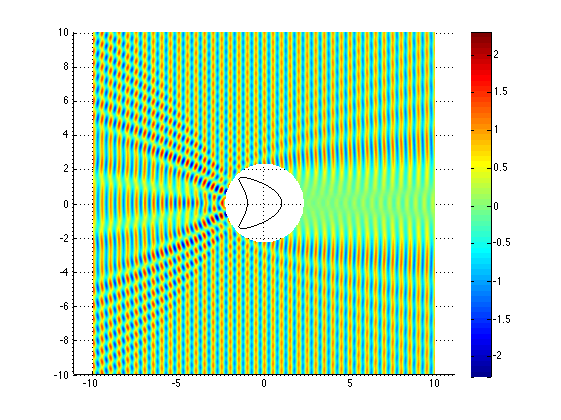
\includegraphics[width=12cm]{kite_totalfield}
\caption{\label{fig:kite_totalfield}
Visualization of the total field induced by a plane wave   impinging  on the kite.}
\end{figure}

\section{Other \texttt{wavefunctionexpansion} operations}\label{sec:add_feat}
The additional features of the TMATROM kernel classes described in this section are useful for 
efficient online simulation of multiple particle configurations with dynamic
locations and orientations of obstacles.
%, such as that in Figure~\ref{fig:multiple_dyn_sim}.



\techheading{Copying}
A !regularwavefunctionexpansion! object
!u! is copied using
\begin{matlab}
v = regularwavefunctionexpansion(u);
\end{matlab}
Similarly,
a !radiatingwavefunctionexpansion! object
!u! is copied using
\begin{matlab}
v = radiatingwavefunctionexpansion(u);
\end{matlab}

\techheading{Changing the expansion origin (regular to regular)}
A regular wave function expansion~(\ref{eq:regular-expansion}) may be
expanded about a new origin using the translation-addition theorem~\cite{dufva}.
The origin of a 
!regularwavefunctionexpansion! object !u! 
is changed to a new origin !x1! using
\begin{matlab}
u.changeorigin(x1)
\end{matlab}
An alternative is to create a new !regularwavefunctionexpansion! object !v!
with origin !x1! using
\begin{matlab}
v = regularwavefunctionexpansion(u,x1);
\end{matlab}
A new !regularwavefunctionexpansion! object !v!
with order !n1! and origin !x1! is created using
\begin{matlab}
v = regularwavefunctionexpansion(u,x1,n1);
\end{matlab}
In all three cases the expansion 
coefficients with respect to the new origin are computed using
the translation addition theorem~\cite{dufva}.



 
\techheading{Changing the expansion origin (radiating to radiating)}
A radiating wave function expansion~(\ref{eq:radiating-expansion}) may be
expanded about a new origin using the translation-addition theorem.
The origin of a 
!radiatingwavefunctionexpansion! object !u! 
is changed to a new origin !x1! using
\begin{matlab}
u.changeorigin(x1)
\end{matlab}
An alternative
is to create a new !radiatingwavefunctionexpansion! object !v!
with origin !x1! using
\begin{matlab}
v = radiatingwavefunctionexpansion(u,x1);
\end{matlab}
A new !radiatingwavefunctionexpansion! object !v!
with order !n1! and origin !x1! is created using
\begin{matlab}
v = radiatingwavefunctionexpansion(u,x1,n1);
\end{matlab}
In all three cases the expansion 
coefficients with respect to the new origin are computed using
the translation addition theorem~\cite{dufva}.

\techheading{Changing the expansion origin (radiating to regular)}
If a radiating wave function expansion~(\ref{eq:radiating-expansion}) is
regular in a neighborhood of the new origin !x1! then it may also be
approximated using a regular wavefunction expansion about the new origin
\begin{matlab}
v = regularwavefunctionexpansion(u,x1);
\end{matlab}
A new !regularwavefunctionexpansion! object !v!
with order !n1! and origin !x1! is created using
\begin{matlab}
v = regularwavefunctionexpansion(u,x1,n1);
\end{matlab}
In both cases the coefficients with respect to the new origin are computed using
the translation addition theorem~\cite{dufva}.

\techheading{Rotating the coordinate system}
A regular wave function expansion~(\ref{eq:regular-expansion}) 
or radiating wave function expansion~(\ref{eq:radiating-expansion}) 
may be expanded 
in a new coordinate system obtained by rotating the old
axes (with origin at the expansion origin).
A !regularwavefunctionexpansion! or 
!radiatingwavefunctionexpansion! object u 
is transformed to a coordinate system rotated by angle !theta! in the 
positive direction using
\begin{matlab}
u.rotatecoordinates(theta)
\end{matlab}

\techheading{Example}
In this example
we use a !radiatingwavefunctionexpansion! object !v! with origin 0 
representing
the field scattered by a kite shaped object.
The field is visualized in Figure~\ref{fig:addition-theorem} (left).

Using the command
\begin{matlab}
v.rotatecoordinates(pi/6)
\end{matlab}
we rotate the coordinate system 
by angle $\pi/6$ in the positive direction.
Subsequent calls to the !evaluate! method will be with respect to 
the new coordinate system.
The field is visualised with respect to the
new coordinate system in Figure~\ref{fig:addition-theorem} (center).

Now
\begin{matlab}
u = regularwavefunctionexpansion(v,4-2i);
\end{matlab}
constructs a !regularwavefunctionexpansion! object !u! 
that represents the field in a neighbourhood of $(4,-2)^T$
(with respect to the rotated coordinate system).
This regular wavefunction expansion is visualised
in Figure~\ref{fig:addition-theorem} (right)
in a ball around $(4,-2)^T$.


\begin{figure}[!ht]
\centering
\begin{tabular}{ccc}
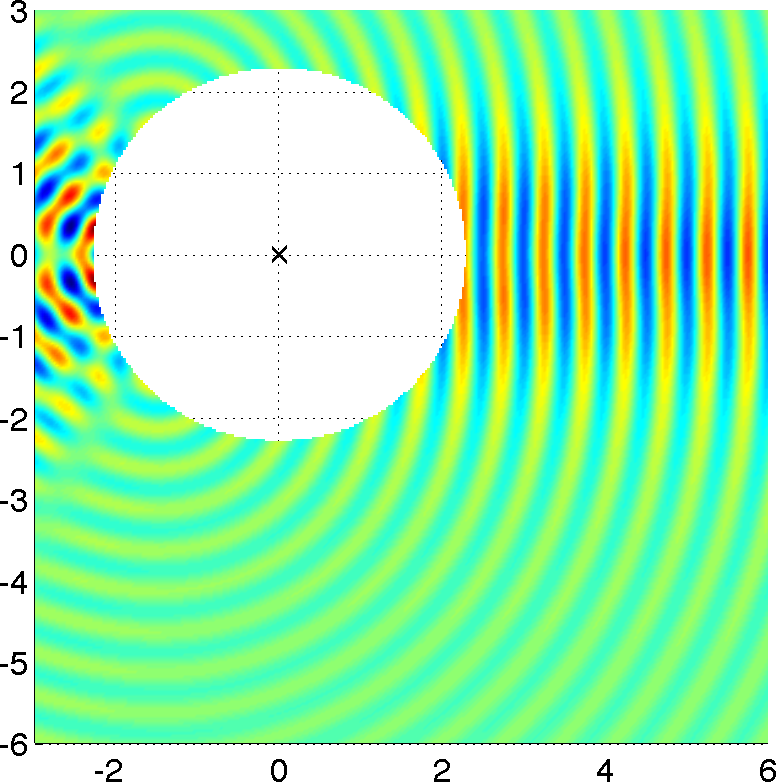
\includegraphics[width=5cm]{addition_theorem_original.png} &
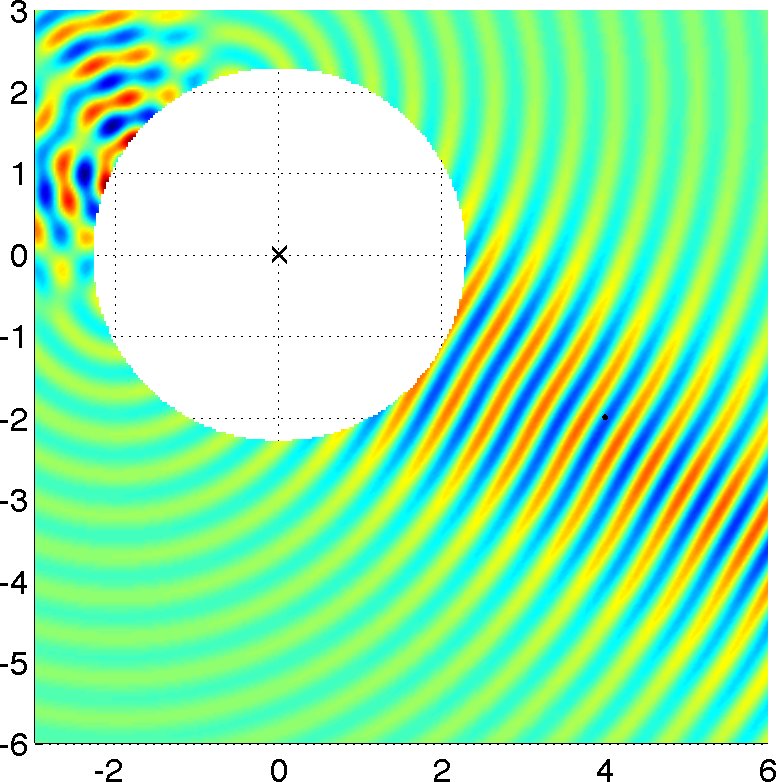
\includegraphics[width=5cm]{addition_theorem_rotated.png} &
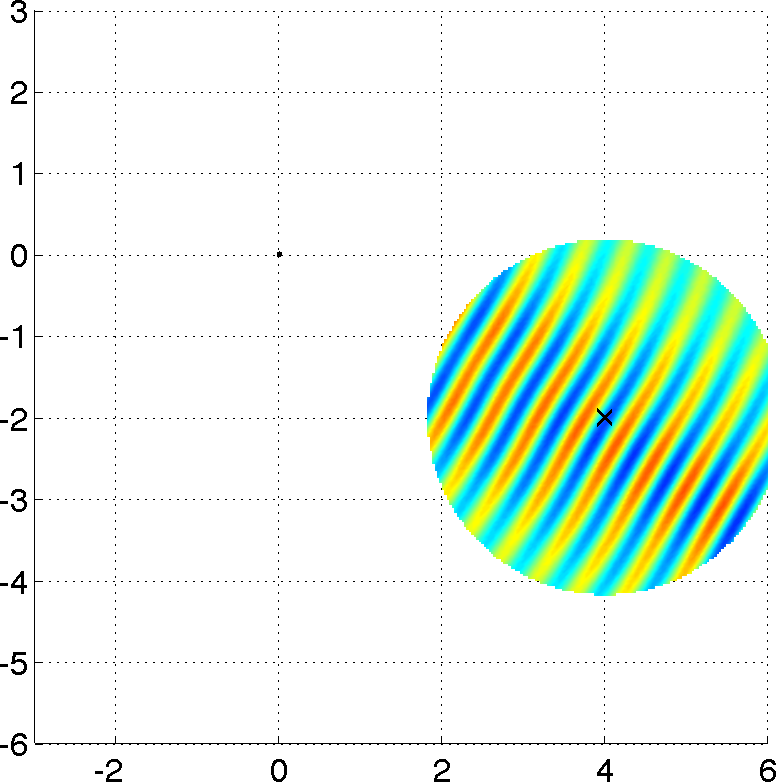
\includegraphics[width=5cm]{addition_theorem_radiating_to_regular.png}
\end{tabular}
\caption{\label{fig:addition-theorem}
Visualizations of a  field scattered by a kite shaped object in the original coordinate system (left);
in a rotated coordinate system (center); and with a new expansion center
$(4,-2)^T$.
The expansion centers are marked with $\times$.}
\end{figure}


\section{The \texttt{tmatrix} class}

Linearity of the Helmholtz equation~\eqref{eq:helmholtz} implies that 
when an incident wave~(\ref{eq:regular-expansion}) is scattered by a configuration, 
the radiating wave expansion coefficients~(\ref{eq:radiating-expansion}) satisfy
\begin{equation}
\label{eq:tmatrix-product}
\underline{b} = T \underline{a},
\end{equation}
where $T$ is a matrix, called the T-matrix.
Here we assume that the 
series are not truncated (so $n=\infty$) and 
$\underline{a} = (a_m)_{m \in \bbN}$,
$\underline{b} = (b_m)_{m \in \bbN}$.
This relation holds approximately when the series expansions are truncated
to a finite order $n$, and the corresponding T-matrix is a 
$(2n+1) \times (2n+1)$ matrix, denoted below as $T_n$. 

\techheading{Instantiation}
The T-matrix 
depends on the scatterer, and on the
center chosen for the wavefunction expansions of the incident 
and scattered waves, but
is independent of their expansion coefficients (and hence the incident field).
The !tmatrix! class represents the T-matrix of a scatterer.
An instance of the !tmatrix! class 
for expansions of order !n! 
is created using
\begin{matlab}
tmat = tmatrix(n,k,s,x0);
\end{matlab}
where !x0! is the expansion origin and !k! is the wavenumber.
The solver !s! is described below.

\techheading{Solver}
The parameter !s! represents a solver (based, for example, on 
various types of boundary and finite element methods)  for  the two dimensional wave
scattering problem described in Section~\ref{sec:model} for a fixed set
of parameters determining the problem. 
The shape (and properties of the scatterer) enter the T-matrix 
through the solver.
Example solvers are provided with the TMATROM package but users can also
setup a solver class based on their own solver for the two dimensional
wave scattering problem.
The solver is explained in more detail in the next section.

\techheading{Error measure to quantify the accuracy of the truncated T-matrix}
The infinite T-matrix $T$ 
satisfies the symmetry relation~\cite[Theorem~1]{gh:tmat2d}
\begin{displaymath}
T + T^* + 2TT^* = 0
\end{displaymath}
in the case of sound-soft, sound-hard or transmission boundary conditions
applied on the scatterer surface.
The symmetry condition also holds in the Robin boundary condition case
under certain conditions on the impedance.
In the case of a truncated T-matrix $T_n$, the quantity
\begin{displaymath}
\max_{\ell,m = -n,\dots,n} | (T_n + T_n^* + 2 T_n T_n^*)_{\ell,m} |
\end{displaymath}
gives a useful measure of the error.
This error measure is computed for a !tmatrix! object !T! using
\begin{matlab}
T.error()
\end{matlab}

The error measure above depends on the solver !s! and also on the order !n! chosen for 
the wavefunction expansions. 
A suitable expression for the order in the case of spherical scatterers is 
given in~\cite{wiscombe:mie}   
and our experience~\cite{gh:ctac-tmatrix, ghh:tmatrix}  suggests that this choice is usually 
suitable for two dimensional circular scatterers and scatterers of other shapes.
This order can be calculated using
\begin{matlab}
n = suggestedorder(k,r);
\end{matlab}
where !r! is the radius of the scatterer.
We refer to~\cite{ghh:tmatrix} for convergence results for the T-matrix.

\techheading{Scattered field computation}
The radiating 
scattered field induced by scattering of an incident field is given by
\begin{matlab}
b = T * a;
\end{matlab}
Here !a! is a !regularwavefunctionexpansion! representing the incident field,
!T! is a !tmatrix!
and !b! is a !radiatingwavefunctionexpansion! representing the scattered field.
The objects !a! and !T! are required to have the same wavenumber,
origin and order.

\techheading{Single particle configuration examples with multiple parameters}
Our source codes
\begin{matlab}
example_rom_nystrom_soundsoft_bistatic.m
example_rom_nystrom_soundsoft_monostatic.m 
example_rom_nystrom_soundhard_bistatic.m
example_rom_nystrom_soundhard_monostatic.m 
example_rom_nystrom_absorbing_bistatic.m
example_rom_nystrom_absorbing_monostatic.m 
\end{matlab}
in the TMATROM subdirectory !EXAMPLE_ROM_NYSTROM_SOLVER! 
illustrate the usage of the !tmatrix! class for multi-parameter scattering
by configurations containing single obstacles with 
various material properties. 

\techheading{Multiple particle configuration simulations using the T-matrix}
Having assembled the T-matrix ROM for each particle in the configuration
we can efficiently simulate scattering by many configurations 
(with the same particles but varying locations and orientations of the particles)
using the additional object oriented features described
in Section~\ref{sec:add_feat}.

To briefly describe the method, we 
consider scattering of an incident field !p! by a configuration
containing three individual particles with centers !x{1}!, !x{2}!
and !x{3}! respectively.
We assume that the T-matrices 
!tmat{1}!, !tmat{2}! and !tmat{3}!
of the three particles have already been computed with origin 0.
Using a logical origin at 0 
corresponds to using local coordinates about the center of each particle.

We let 
!a{1}!, !a{2}! and !a{3}! be the radiating wavefunction expansions of the 
field scattered by the three particles.
Then the scattered field is !a{1} + a{2} + a{3}! and the total field is
!p + a{1} + a{2} + a{3}!.

Let us consider what happens on the first scatterer, which has center
!x{1}!.
The incident field on the first particle consists of the incident wave !p!
and the field !a{2} + a{3}! scattered by the other particles.
We can combine these into a single regular wavefunction expansion with 
center !x{1}!
\begin{matlab}
regularwavefunctionexpansion(n,x{1},p) ...
       + regularwavefunctionexpansion(a{2},x{1}) ...
       + regularwavefunctionexpansion(a{3},x{1})
\end{matlab}
where !n! is the order of the wavefunction expansions.

The scattered field can then be computed from the incident field
using the T-matrix.
To facilitate this we first set the logical origin of the T-matrix to
be the center of the first particle
\begin{matlab}
tmat{1}.setOrigin(x{1});
\end{matlab}
Then the scattered field is computed from the incident field in the usual
way
\begin{matlab}
a{1} = tmat{1} * ( regularwavefunctionexpansion(n,x{1},p) ...
       + regularwavefunctionexpansion(a{2},x{1}) ...
       + regularwavefunctionexpansion(a{3},x{1}) );
\end{matlab}

In practice the radiating wavefunction expansions !a{1}!, !a{2}! and !a{3}!
are unknown.
However, the expression above, and similar expressions derived for
the other scatterers, give a linear system for the radiating wavefunction
expansion coefficients that can be solved iteratively.
In the example
\begin{matlab}
example_rom_nystrom_multiple_config.m
\end{matlab}
the linear system is solved using GMRES.

For the full algorithm and the corresponding mathematical description,
including full details of the linear system and its solution, 
we refer to~\cite[Section 2.2]{gh:stoc_mult}. Details in the source code 
\begin{matlab}
example_rom_nystrom_multiple_config.m
\end{matlab}
in the TMATROM subdirectory !EXAMPLE_ROM_NYSTROM_SOLVER! 
illustrate the ROM simulation and reproduce the visualisations of the scattered and total field in
Figure~\ref{fig:multiple_ex_sim} for the multiple particle configuration model.
The preliminary off line step is to 
build the T-matrix ROM for each distinctly shaped template particle in the configuration. 
This approach
is easily adapted for simulating dynamic multiple particle configurations. 


%\vspace{-1.2in}
\begin{figure}[ht!]
\centering
\begin{tabular}{ll}
\hspace{-0.5in}
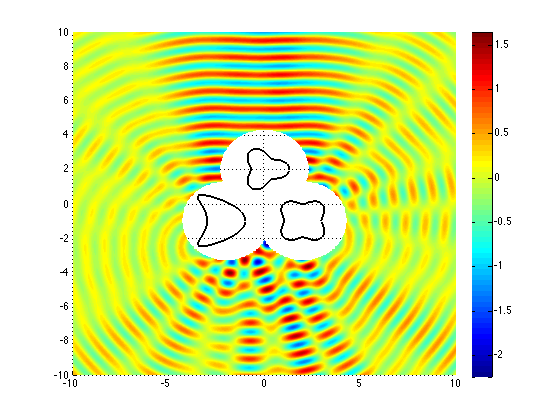
\includegraphics[width=10cm]{multiple_kpt_realscat_field} & \hspace{-1.0in} 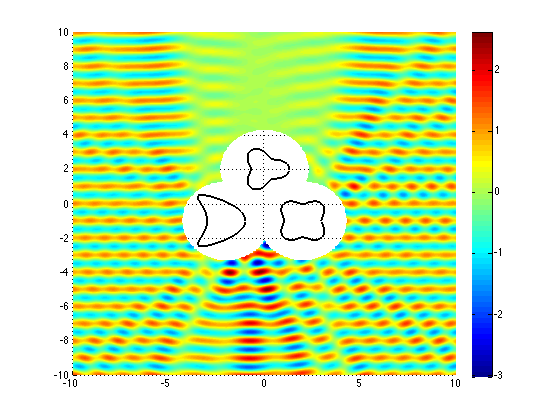
\includegraphics[width=10cm]{multiple_kpt_total_field} \\
\end{tabular}
\caption{\label{fig:multiple_ex_sim}
Multiple-parameter acoustic computer model  using ROM scattering characterization (independent of the location, orientation, input incident wave, and output observation direction) of  each distinctly shaped particle.   
Real part of scattered field (left) and  total field (right) of  a multiple particle configuration.}
\end{figure}


\part{Using the provided solvers}
\label{part:provided-solvers}

\section{The \texttt{solverNystrom} sound soft  scatterer solver}

The !solverNystrom! class solves the scattering 
problem~\eqref{eq:helmholtz}--\eqref{eq:radiation-condition} 
for a single particle $D$
subject
to the sound soft boundary condition
\begin{displaymath}
u(\x) + u^\mathrm{i}(\x) = 0, \qquad \x \in \surface,
\end{displaymath}
where $\surface$ denotes the boundary of the particle.
The boundary integral equation reformulation of the scattering problem 
and its solution using the high order Nystr\"om method is described
in~\cite[Section~3.5]{colton:inverse}.

\techheading{Example boundaries}
The boundary $\surface$ is represented by an object of class !obstacle!.
Some example obstacle classes are provided in the TMATRIX package, including
the circle with radius !r!,
\begin{matlab}
b = obstacleCircle(r);
\end{matlab}
the kite  shaped obstacle~\cite[Page~79]{colton:inverse}, 
\begin{matlab}
b = obstacleKite();
\end{matlab}
the pinched ball~\cite[Page~94]{colton:inverse}
\begin{matlab}
b = obstaclePinchedBall();
\end{matlab}
the cylinder with height !h! and width !w! capped with semi-circles
\begin{matlab}
b = obstacleCappedCylinder(h,w);
\end{matlab}
and the trefoil~\cite{mpspack:manual}
\begin{matlab}
b = obstacleTrefoil();
\end{matlab}

\techheading{Polar coordinate boundaries}
Obstacles described by polar coordinates can easily be represented using
\begin{matlab}
b = obstaclePolar(r,dr,ddr);
\end{matlab}
where the anonymous functions !r!, !dr! and !ddr! represent the radius function
and its first and second derivatives with respect to !t!.
For example, the pinched ball is given by
\begin{matlab}
r = @(t) sqrt(1.44 - 0.5*cos(-4*t));
dr = @(t) -sin(-4*t)./sqrt(1.44 - 0.5*cos(-4*t));
ddr = @(t) -sin(-4*t).^2./(1.44 - 0.5*cos(-4*t)).^1.5 ...
           + 4*cos(-4*t)./sqrt(1.44 - 0.5*cos(-4*t));
b = obstaclePolar(r,dr,ddr);
\end{matlab}

\techheading{Instantiation}
A !solverNystrom! object is created using
\begin{matlab}
S = solverNystrom(k,[],b);
\end{matlab}
where !k! is the wavenumber and !b! is an obstacle.
The incident field(s) are then set using
\begin{matlab}
S.setIncidentField(inc)
\end{matlab}
where !inc! is a cell array of !incident! objects.
For example
\begin{matlab}
inc{1} = plane_wave(0,k);
inc{2} = point_source(3+2i,k);
S.setIncidentField(inc);
\end{matlab}
sets two incident fields, the first induced by a plane wave and the second
induced by a point source.

\techheading{Solving}
The integral operators are discretized 
using the Nystr\"om scheme with 2!q! quadrature points 
using
\begin{matlab}
S.setup(q)
\end{matlab}
and the corresponding linear systems are solved using
\begin{matlab}
S.solve();
\end{matlab}

\techheading{Far field computation}
The far field is then obtained at points with angle 
specified in the vector !theta! using
\begin{matlab}
F = S.getFarField(theta,[1 2]);
\end{matlab}
Here !F(:,1)! is the far field corresponding to !inc{1}! and
!F(:,2)! is the far field corresponding to !inc{2}!.

\techheading{Example}
A full example to simulate scattering of a plane wave and spherical wave
induced by a point source impinging on a sound soft pinched ball shaped scatterer is below. 
The resulting  simulated intensity of far fields are visualized in Figure~\ref{fig:solver}.
\begin{matlab}
b = obstaclePinchedBall();
k = 1;
q = 15;
S = solverNystrom(k,[],b);
inc{1} = plane_wave(0,k);
inc{2} = point_source(3+2i,k);
S.setIncidentField(inc);
S.setup(q)
S.solve();
theta = linspace(0,2*pi);
F = S.getFarField(theta,[1 2]);
plot(theta,10*log10(2*pi*abs(F(:,1)).^2),'r*')
hold on
plot(theta,10*log10(2*pi*abs(F(:,2)).^2),'mo')
legend('input:planewave', 'input:pointsource') 
axis([0 2*pi -2 14])
\end{matlab}

\begin{figure}
\centering
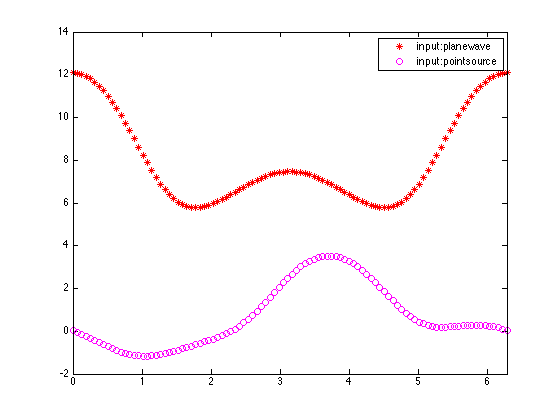
\includegraphics[width=10cm]{solver_pinched_ball.png}
\caption{\label{fig:solver}
Visualization of the ACS of a pinched ball with incident plane
wave  and point source circular wave.
}
\end{figure}

\section{The \texttt{solverNystromRobin} for simulating scattering models
with sound-hard (Neumann) or absorbing (Robin) boundary conditions }

The !solverNystromRobin! class solves the scattering 
problem~\eqref{eq:helmholtz}--\eqref{eq:radiation-condition} for a single particle $D$ subject
to the Robin boundary condition
\begin{displaymath}
\frac{\partial\ }{\partial n} (u+u^\mathrm{i})(\x) + i \mu (u+u^\mathrm{i})(\x) = 0, \qquad \x \in \surface,
\end{displaymath}
where $\surface$ denotes the boundary of the particle.
Here $\mu$ is the Robin boundary condition parameter.
The case $\mu=0$ is equivalent to the sound-hard boundary condition.
%The boundary integral equation reformulation of the scattering problem 
%and its solution using the high order Nystr\"om method is described
%in~\cite{kirsch:coupled}.

\techheading{Instantiation}
A !solverNystromRobin! object is created using
\begin{matlab}
S = solverNystromRobin(k,[],b,mu);
\end{matlab}
where !k! is the wavenumber, !b! is an obstacle and
!mu! is the Robin boundary condition parameter.

\techheading{Other methods}
Usage of the !solverNystromRobin! object after it is created is identical to
the usage of the !solverNystrom! object described in the previous section.

\part{Incorporating a user defined solver}
\label{part:solvers-user}

\section{The solver class}

\techheading{Abstract methods}
The !tmatrix! class is instantiated with an object of class !solver!.
In practice this object must be an instance of a class derived from
!solver! and the derived class must provide methods with interfaces
\begin{matlab}
setup(self)
solve(self)
val = getFarField(self,points,index)
\end{matlab}
We have provided the !solver! class and we recommend that user defined
solvers are derived from the !solver! class using
\begin{matlab}
classdef my_solver < solver
\end{matlab}
syntax.
The methods above are declared as abstract methods in the !solver! class and 
hence they must be overwritten in the child class.
We have found that provision of !setup! and !solve! methods facilitates
easy extension of solver classes.
Before expanding on the !setup! and !solve! methods we discuss 
some other methods of the !solver! class.

\techheading{Constructor}
The constructor for the !solver! class has interface
\begin{matlab}
obj = solver(kwave,incidentField)
\end{matlab}
Here !kwave! is the wavenumber.
It is expected that the solver be able to solve several 
scattering problems arising from several incident fields.
The incident fields are given as a cell array 
!incidentField! and each item in the cell array should be of type !incident!.
Incident fields are discussed in the next section.

The command
\begin{matlab}
obj = solver(kwave,[])
\end{matlab}
defers setting the incident field.
The incident field can be set subsequently using
\begin{matlab}
obj.setIncidentField(incidentField)
\end{matlab}
The incident fields are again given as a cell array 
!incidentField! and each item in the cell array should be of type !incident!.
Incident fields are discussed in the next section.

\techheading{Visualization}
The !solver! class also provides methods for plotting the far field and 
cross section. We refer to !help solver! for full details.

\techheading{\texttt{setup} method}
The solver is setup using
\begin{matlab}
obj.setup();
\end{matlab}
This method would typically perform tasks that are performed once only,
such as computing a discretization matrix.

\techheading{\texttt{solve} method}
The solver is applied using
\begin{matlab}
obj.solve();
\end{matlab}
This method would typically perform tasks that
depend on the incident wave.
For example, this method might solve a linear system 
(with the discretization matrix)
for each of several right hand sides that are derived from several given incident fields.

\techheading{\texttt{getFarField} method}
The far field corresponding to the incident fields 
is computed from
a !solver! object !obj! using
\begin{matlab}
val = obj.getFarField(points,index)
\end{matlab}
Here !points! is a vector of angles in $[0,2 \pi]$ 
and
!val! is matrix with !val(:,k)! being the values of the far field
induced by the incident field !incidentField{index(k)}! at
the observation angles specified in !points!.

\techheading{Example}
The user is free to define the !setup!, !solve! 
and !getFarField! methods any way that they like as long as the above 
functionality is provided.

A typical structure is seen in the class !solverNystrom! which is provided as
an example.
The !setup! method creates a matrix representing the operators in an 
integral equation.
The !solve! method solves the linear system associated with the
integral equation for each 
incident field and stores the coefficients.
The !getFarField! method computes the far field for each incident field
using the stored coefficients.

\techheading{Extension}
Finally, we note that the user is free to specify further useful methods in their
solver class.
For example, in the !solverNystrom! class we have specified further methods for
visualizing the scattering obstacle and determining its radius.

\techheading{Online documentation}
Full documentation of !solverNystrom! is obtained using
\begin{matlab}
help solverNystrom
\end{matlab}

\techheading{Template}
A template for a user defined solver is given in !solver_template.m!.

\section{Details of incorporating a user defined solver}

In this section we work through an example of constructing a user defined
!solver! class. 
All that is required of the solver is that it can compute the far field 
corresponding to a given incident field.

In this example we show how to construct a !solver! class 
using the 
MPSPACK~\cite{mpspack:manual} solver.
Before describing our !solver! class, we give a simple 
example of using MPSPACK to solve a single scattering problem for a 
sound soft scatterer described using polar coordinates.
For brevity, we will use this code with minimal explanation, and we refer
to the MPSPACK manual~\cite{mpspack:manual} for full details of how to
use MPSPACK.
Understanding how to solve a single scattering problem using MPSPACK will make it easy to see
how the associated solver class works.

We will mainly focus on the details related to incorporating the solver MPSPACK into 
the object oriented framework of TMATROM. Below we assume that the user has downloaded the
MPSPACK solver in a directory and added the directory to the Matlab path.
To verify that MPSPACK is installed correctly
we recommend that the user types the following two commands 
\begin{matlab}
example_rom_mpspack_soundsoft_bistatic
example_rom_mpspack_soundhard_bistatic
\end{matlab}

First we setup the MPSPACK solver.
The main tasks are to describe the boundary of the scatterer by specifying
function handles !f! and !df! that give the radius and its derivative as a 
function of angle.
These functions can be defined as anonymous functions.
Then an instance of the MPSPACK !scattering! class is created
and stored as !scatteringObject! and the wavenumber is set.
\begin{matlab}
kwave = 1;
tau = 0.1;
n = 100;
m = 2*n;
opts= struct('eta',kwave,'fast',2,'multiplier',2.1,'tau',tau);
boundary = segment.radialfunc(m, {f,df});
boundary.setbc(1,'D', []);
d = domain([], [], boundary, -1);
d.addmfsbasis(boundary,n,opts);
scatteringObject = scattering(d, []);
scatteringObject.setoverallwavenumber(kwave);
\end{matlab}
The next part depends on the incident wave.
Here we consider an incident wave stored as !inc! which is of type incident.
For example
\begin{matlab}
inc = plane_wave(pi/4,kwave);
\end{matlab}
We define anonymous functions !ui!, !uix! and !uiy! 
that evaluate the incident field, and the $x$- and $y$-coordinates of its
gradient respectively.
These are required by MPSPACK for simulating scattering of the incident wave.

Using these we call the !setincidentwave! method of !scattering!.
Finally we call the !solvecoeffs! method of !scattering!, which solves
a linear system to obtain a vector of coefficients.
This vector of coefficients depends on the incident wave.
We need to know that this vector is stored as !scatteringObject.co!,
but it is internal
to MPSPACK and we do not need to understand its true meaning.
\begin{matlab}
ui = @(x) inc.evaluate(x);
uix = @(x) inc.evaluateGradient(x);
f = @(x) inc.evaluateGradient(x);
uiy = @(x) getSecondOutput(f,x);
scatteringObject.setincidentwave(ui,uix,uiy);
scatteringObject.solvecoeffs;
\end{matlab}
Finally we compute the far field at points specified in the vector !points!.
For example
\begin{matlab}
points = linspace(0,2*pi,100);
\end{matlab}
This computation uses the MPSACK internal vector 
!scatteringObject.co!.
\begin{matlab}                
farfield = scatteringObject.gridfarfield(opts,points);
\end{matlab}
It is clear that the computation of the far field breaks down into three distinct stages.
The first is a setup stage that is independent of the incident field.
The second is a solve stage that computes some internal quantity that
depends on the incident field.
The third stage is the far field computation.
These three stages form the basis of the
!setup!, !solve! and !getFarField! methods in our solver class.
These are the methods that are declared as abstract in the !solver! base
class.

\techheading{class definition}
We begin by creating a file !mfsExampleSolver.m! that contains the class
declaration for our !mfsExampleSolver! class.

First we declare our new class !mfsExampleSolver! as a child of the
!solver! class. 
\begin{matlab}
classdef mfsExampleSolver < solver

    % subsequent code will be inserted here

end
\end{matlab}
This means that the child !mfsExampleSolver! inherits several methods and 
properties
that are defined in the parent !solver! class.
In addition to these, the !mfsExampleSolver! solver class needs several
properties of its own, which are mainly parameters for the MPSPACK solver.
\begin{matlab}
classdef mfsExampleSolver < solver

    properties
        f
        df
        scatteringObject
        tau
        m
        n
        coeffs
    end
    
    % subsequent code will be inserted here

end
\end{matlab}
The !mfsExampleSolver! class also needs several methods.
For now we give a template code. We will expand the function definitions below.
\begin{matlab}
classdef mfsExampleSolver < solver

    properties
       ...
    end
    
    methods

        function self = mfsExampleSolver(kwave,incidentField,f,df,n,tau,m)
            ...
        end

        function setup(self)
            ...
        end

        function solve(self)
            ...
        end

        function val = getFarField(self,points,index)
            ...
        end

    end

end
\end{matlab}

\techheading{\texttt{mfsExampleSolver} constructor}
First we declare the class constructor function, which must have the
same name as the class.
In this example we take the MPSPACK parameters as parameters of the 
constructor function.
\begin{matlab}
function self = mfsExampleSolver(kwave,incidentField,f,df,n,tau,m)
\end{matlab}
Our first task in the constructor
is to create the object !self! by calling the parent 
class constructor function. The object !self! is then instantiated as
!mfsExampleSolver! class.
\begin{matlab}                        
    self = self@solver(kwave,incidentField);           
\end{matlab}
Our next task is to copy the given parameters into the class properties.
\begin{matlab}
    self.f = f;
    self.df = df;
    self.m = m;
    self.n = n;
    self.tau = tau;
\end{matlab}
Finally, we set to empty the !scatteringObject! and !coeffs! properties
of !self!.
These properties will be set later by other methods.
\begin{matlab}
    self.scatteringObject = [];
    self.coeffs = [];
\end{matlab}

\techheading{\texttt{setup} method}
We assume that all of the parameters for the !mfsExampleSolver! are set
in the constructor, so that the setup method has no parameters.
\begin{matlab}
function setup(self)
\end{matlab}
Now the function body contains essentially the same code we used to setup
our MPSPACK example.
Note that we now use our class properties for the parameters.
\begin{matlab}
    opts= struct('eta',self.kwave,'fast',2,'multiplier',2.1,'tau',self.tau);
    boundary = segment.radialfunc(self.m, {self.f,self.df});
    boundary.setbc(1,'D', []);
    d = domain([], [], boundary, -1);
    d.addmfsbasis(boundary,self.n,opts);
\end{matlab}
Finally, the MPSPACK !scattering! object is stored in the 
!scatteringObject! property of !self! so that it can be accessed from 
other methods.
\begin{matlab}
    self.scatteringObject = scattering(d, []);
    self.scatteringObject.setoverallwavenumber(self.kwave);
\end{matlab}

\techheading{\texttt{solve} method}
Again we assume that all of the parameters for the !mfsExampleSolver! are set
in the constructor, so that the setup method has no parameters.
\begin{matlab}
function solve(self)
\end{matlab}
As before, we closely follow the code we used in the MPSPACK example above.
The main difference is that we need to solve for each of several incident 
fields given in the cell array !self.incidentField!.
This necessitates a loop through the cell array.
\begin{matlab}
    for k=1:length(self.incidentField)
\end{matlab}
Now we essentially repeat the code from the MPSPACK example above.
\begin{matlab}                
        ui = @(x) self.incidentField{k}.evaluate(x);
        uix = @(x) self.incidentField{k}.evaluateGradient(x);
        f = @(x) self.incidentField{k}.evaluateGradient(x);
        uiy = @(x) getSecondOutput(f,x);                
        self.scatteringObject.setincidentwave(ui,uix,uiy);
\end{matlab}
In the MPSPACK example above we solved for only a single incident field
and we could assume that MPSPACK internal variables were in the correct
state.
In this code we must reset the MPSPACK internal variable !rhs! ourselves.
\begin{matlab}    
        self.scatteringObject.rhs = [];                
\end{matlab}
Now we can solve the MPSPACK linear system using the MPSPACK !solvecoeffs! 
method.
\begin{matlab}
        self.scatteringObject.solvecoeffs;                
\end{matlab}
Finally we store the MPSPACK internal coefficients in our !coeffs! array
so that we can access it later in other methods.
\begin{matlab}
        self.coeffs{k} = self.scatteringObject.co;                
\end{matlab}

\techheading{\texttt{getFarField} method}
The !getFarField! method is called by the !tmatrix! class and so its interface
cannot be changed. 
The interface is
\begin{matlab}
        function val = getFarField(self,points,index)
\end{matlab}
where !points! is a vector of angles in $[0,2 \pi]$ and index is
an array of integers between 1 and !length(self.incidentField)!.
The return variable !val! is an array of size !length(points)!
by !length(index)! and on return, the !k!th column of !val! must contain the
far field corresponding to !self.incidentField(index(k))!
at the observation angles specified in !points!.

We begin looping through the vector !index!
\begin{matlab}                       
    for k=1:length(index)
\end{matlab}
Our first task is to extract the coefficients corresponding to the
!index(k)!th incident wave from the !coeffs! property and set the
MPSPACK internal variable !co! appropriately.
\begin{matlab}
        self.scatteringObject.co = self.coeffs{index(k)};
\end{matlab}
Then we follow the MPSPACK example above to compute the far field values.
\begin{matlab}
        opts = [];
        val(:,k) = self.scatteringObject.gridfarfield(opts,points);
\end{matlab}

\techheading{Example codes} 
The full code for this example is given in !mfsExampleSolver.m! and
an example of its use is given in !example_user_solver.m! in the   subdirectory !EXAMPLE_ROM_MPSPACK_SOLVER!. 
In the full code we include a small amount of additional code (to 
allow default parameter values and some checking of parameters in methods)
that we omitted above. 

Finally, we remark that reuse of code can be facilitated by using more
complicated nesting of child and parent classes than in the example above.
In the classes
!mfsPolarSoftSolver.m!,
!mfsPolarHardSolver.m!,
!mfsPolarSolver.m!, and
!mfsSolver.m!
we provide an alternative implementation of MPSPACK solvers that facilitates
code reuse for sound soft and sound hard scattering problems and
also for geometries with more general description than polar coordinate
parametrization. Using the above involved structure, we provide two examples in
the subdirectory: 
!example_rom_mpspack_soundsoft_bistatic.m! and !example_rom_mpspack_soundhard_bistatic.m!.

\section{Incident fields}

We assume that the solver can compute the far field of a given incident
field provided it can compute the value of the incident field and its
gradient at appropriate points specified by the solver.

The classes !plane_wave!, !point_source! and 
!regularwavefunction2d! represent common incident fields.

\techheading{Plane wave}
A !plane_wave! object with wavenumber !k! and direction
!exp(1i*theta)! is created using
\begin{matlab}
p = plane_wave(theta,k);
\end{matlab}

\techheading{Point source}
A !point_source! object with wavenumber !k! and point source location !x!
is created using
\begin{matlab}
p = point_source(x,k);
\end{matlab}

\techheading{Regular wave function (incident field)}
A !regularwavefunction2d! object with wavenumber !k!, order !n!
and expansion origin !x0! is created using
\begin{matlab}
p = regularwavefunction2d(n,k,x0);
\end{matlab}

\techheading{Evaluating}
An incident field !p! is evaluated at points !z! using
\begin{matlab}
val = p.evaluate(z);
\end{matlab}
Here !z! may be a scalar, vector or matrix.

\techheading{Evaluating the gradient}
The gradient of an incident field !p!
is evaluated at points !z! using
\begin{matlab}
[dx,dy] = p.evaluateGradient(z);
\end{matlab}
Here !dx! and !dy! are the first and second components of the gradient,
that is, the partial derivatives of the incident field with respect to
$x$ and $y$ respectively.

We remark here the gradient of the incident field is a complex valued vector 
and hence the convention that we use elsewhere,
of using complex values to represent real valued vectors, cannot be used.
This is why we split the components of the gradient into !dx! and !dy!.


%\vspace{-0.2in}
\section*{Acknowledgments}
Support of the National Science Foundation (NSF) and
Colorado Golden Energy Computing Organization (GECO) are gratefully acknowledged.

%\vspace{-0.2in}
\bibliography{references}


\end{document}
